\chapter{向量}
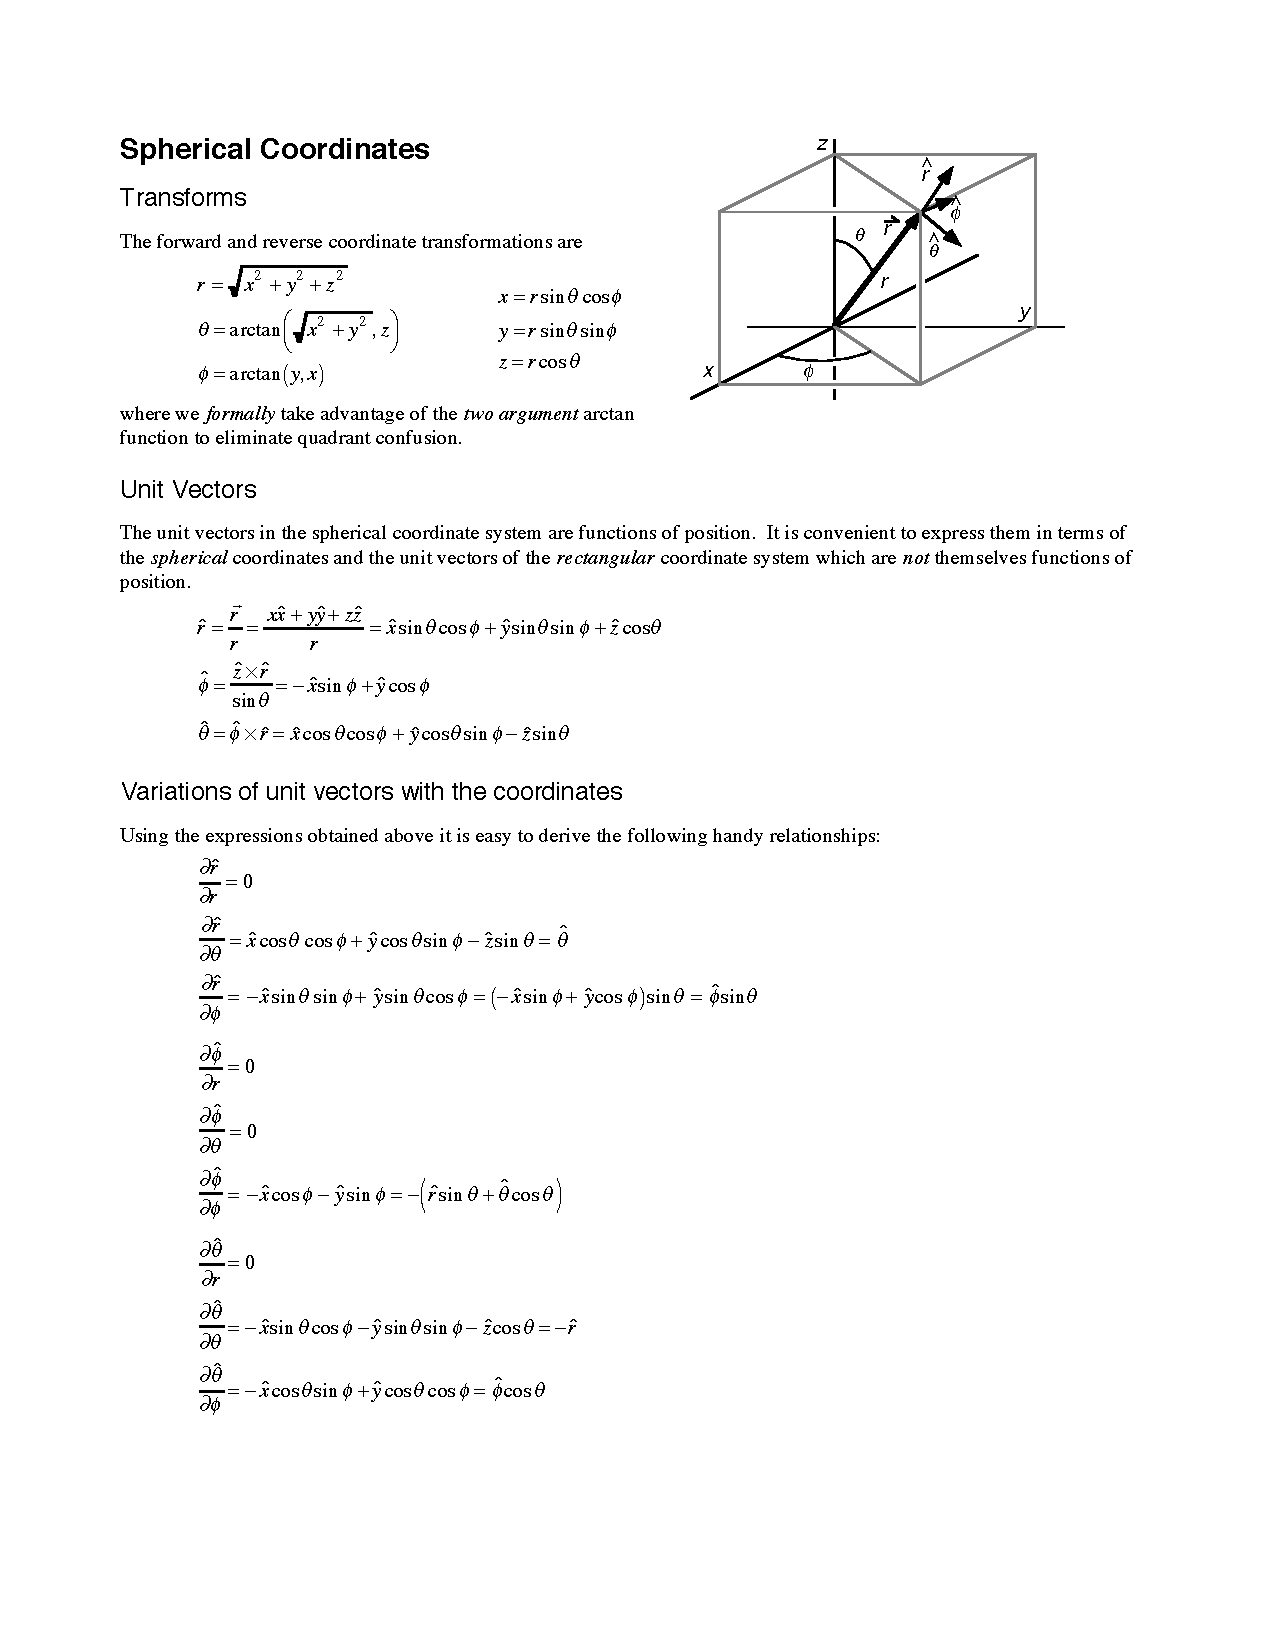
\includepdf[addtotoc={1,section,1,球坐标,cc},pages=1-5]{pdf/Spherical Coordinates.pdf}
\chapter{特征值问题}
\section{1}
\chapter{傅里叶变换}
\section{傅里叶级数}
魏尔斯特拉斯定理告诉我们任意关于x的连续函数都可以展开成x的代数多项式。这个结论可以推广到n个自变量的情形：
\begin{theorem}[Generalized Stone-Weierstrass Theorem]
    如果函数$f(x_1,x_2,\cdots,x_n)$是区间$[a_i,b_i]^n$上的连续函数，那么$f(x_1,x_2,\cdots,x_n)$可以展开成多项式$x_1^{k_1}x_2^{k_2}\cdots x_n^{k_n},k_i\text{是非负整数}$.
\end{theorem}
由$x_1=x=r\cos\theta,x_2=y=r\sin\theta$，我们得到了极坐标下展开一个二元函数的方法：
\begin{align}
    f(r,\theta)=\sum_{m,k=0}^{\infty}a_{mk}x^ky^m=\sum_{m,k=0}^{\infty}a_{m,k}r^{m+k}\cos^k\theta\sin^m\theta
\end{align}
如果我们令$r=1$（或者其他常数）就得到了一个只关于$\theta$的函数：
\begin{align}
    f(\theta)=\sum_{n=-\infty}^{\infty}F_ne^{in\theta}
    =F_0+\sum_{n=1}^{\infty}(A_n\cos\theta+B_n\sin\theta)
\end{align}
这是一个周期为$2\pi$的周期性函数，它可以表示$[-\pi,\pi]$上的连续函数（或者分段连续函数，准确地讲是满足狄利克雷条件的函数）。
利用正交性和归一性，不难求出\cite{Ha}:
\begin{align}
F_n=\frac{1}{2\pi}\int_{-\pi}^{\pi}e^{-in\theta}f(\theta) \dd{\theta}
\end{align}
但是，我们感兴趣的函数并不总是定义在$[-\pi,\pi]$上。更一般的，对于定义在$(a,b)$上，周期为L=(b-a)的函数f(x),通过换元
\begin{align*}
    \theta =\frac{2\pi}{L}(x-a-\frac{L}{2})
\end{align*}
可以得到
\begin{align}
    &f(x)=\sum_{-\infty}^{\infty}F_n e^{2\pi inx/L}\\
    &F_n=\frac{1}{L}\int_{a}^{b}e^{-2\pi inx/L}f(x)\dd{x}
\end{align}
\begin{figure}
    \subfloat[The function we want to represent. (b) The Fourier series representation of
    the function]{
        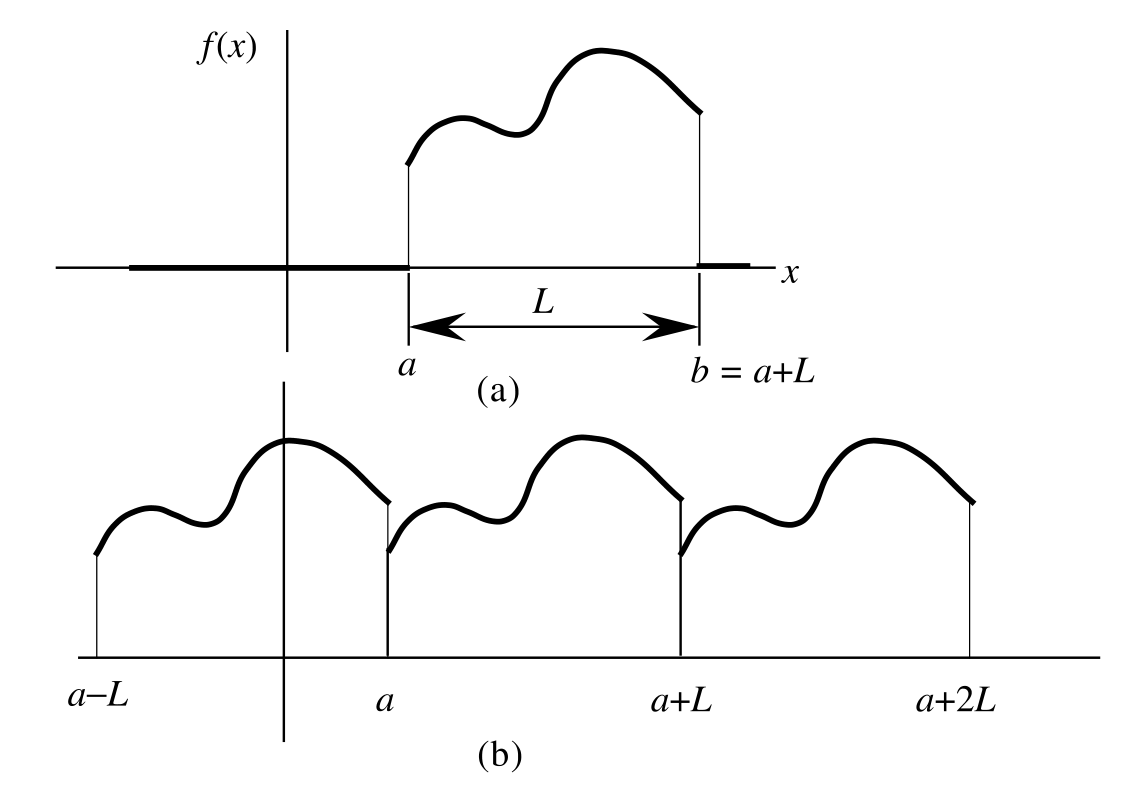
\includegraphics[width=0.45\linewidth]{figure/math/FT.png}
    }
\end{figure}
\section{傅里叶变换}
傅里叶级数可以展开任意周期性函数F(x),但是物理学中遇到的大多数函数并不是周期性的。一种简单的想法是使周期$L\rightarrow \infty$,此时$\Delta\omega=\frac{2\pi}{L}\rightarrow 0$。\cite{MP}我们直接给出傅里叶变换的定义
\begin{align}
    F[f(x)]&=G(\omega)=\int_{-\infty}^{\infty} f(x)e^{-i\omega x}\dd{x}\label{F}\\
    F^{-1}[G(\omega)]&=f(x)=\frac{1}{2\pi}\int_{-\infty}^{\infty}G(\omega)e^{i\omega x}\dd{\omega}\label{-F}
\end{align}
我们称公式\ref{F}为函数f(x)的傅里叶变换,$F[f(x)]=G(\omega)$称为f(x)的像函数.公式\ref{-F}称为$G(\omega)$的傅里叶逆变换,f(x)称为$G(\omega)$的像原函数.
\paragraph{}
上面的定义可以推广到三维:
\begin{align}
    &G(\mbf{\omega})=\int_{-\infty}^{\infty} f(\mbf{r})e^{-i\mbf{\omega\cdot r} }\dd{\mathbf{r}}\\
    &f(\mbf{r})=\frac{1}{2\pi}\int_{-\infty}^{\infty}G(\mbf{\omega})e^{i\mbf{\omega\cdot r}}\dd{\mbf{\omega}}
\end{align}
其中:
\[\begin{cases}
    \mathbf{\omega}=\omega_1\mathbf{e}_1+\omega_2\mathbf{e}_2+\omega_3\mathbf{e}_3\\
    \mathbf{r}=x\mathbf{e}_1+y\mathbf{e}_2+z\mathbf{e}_3\\
    \dd{\mathbf{r}}=\dd{x}\dd{y}\dd{z}\\
    f(\mathbf{r})=f(x,y,z)
\end{cases}\]
\subsection{傅里叶变换的性质}
\begin{itemize}
    \item 线性性质:$F[\alpha f_1+\beta f_2]=\alpha F[f_1]+\beta F[f_2]$.
    \item 延迟性质:$F[e^{i\omega_0x}f(x)]=G(\omega-\omega_0)$.
    \item 位移性质:$F[f(x-x_0)]=e^{-i\omega x_0}F[f(x)]$.
    \item 相似性质:$F[f(ax)]=\frac{1}{|a|}G(\frac{\omega}{a})$.
    \item 微分性质:$F[f^{(n)}(x)]=(i\omega)^nF[f(x)]$,正是由于傅里叶变换的微分性质,引出了求解微分方程的积分变换法.
    \item 积分性质:$F[\int_{x_0}^{x}f(\xi)\dd\xi]=\frac{1}{i\omega}F[f(x)]$.
    \item 卷积性质:$f_1(x)*f_2(x)=\int_{-\infty}^{\infty}f_1(x)f_2(x-\xi)\dd\xi$称为卷积,卷积满足交换律、结合律、分配律。
            对函数和像函数：
            \begin{gather}
                F[f_1(x)*f_2(x)]=F[f_x(x)]\cdot F[f_2(x)]\quad\text{(卷积定理)}\\
                F[f_x(x)\cdot f_2(x)]=\frac{1}{2\pi}F[f_1(x)]*F[f_2(x)]
            \end{gather}
\end{itemize}
